\section{Background and Motivation}\label{background}

\begin{figure}
    \centering
    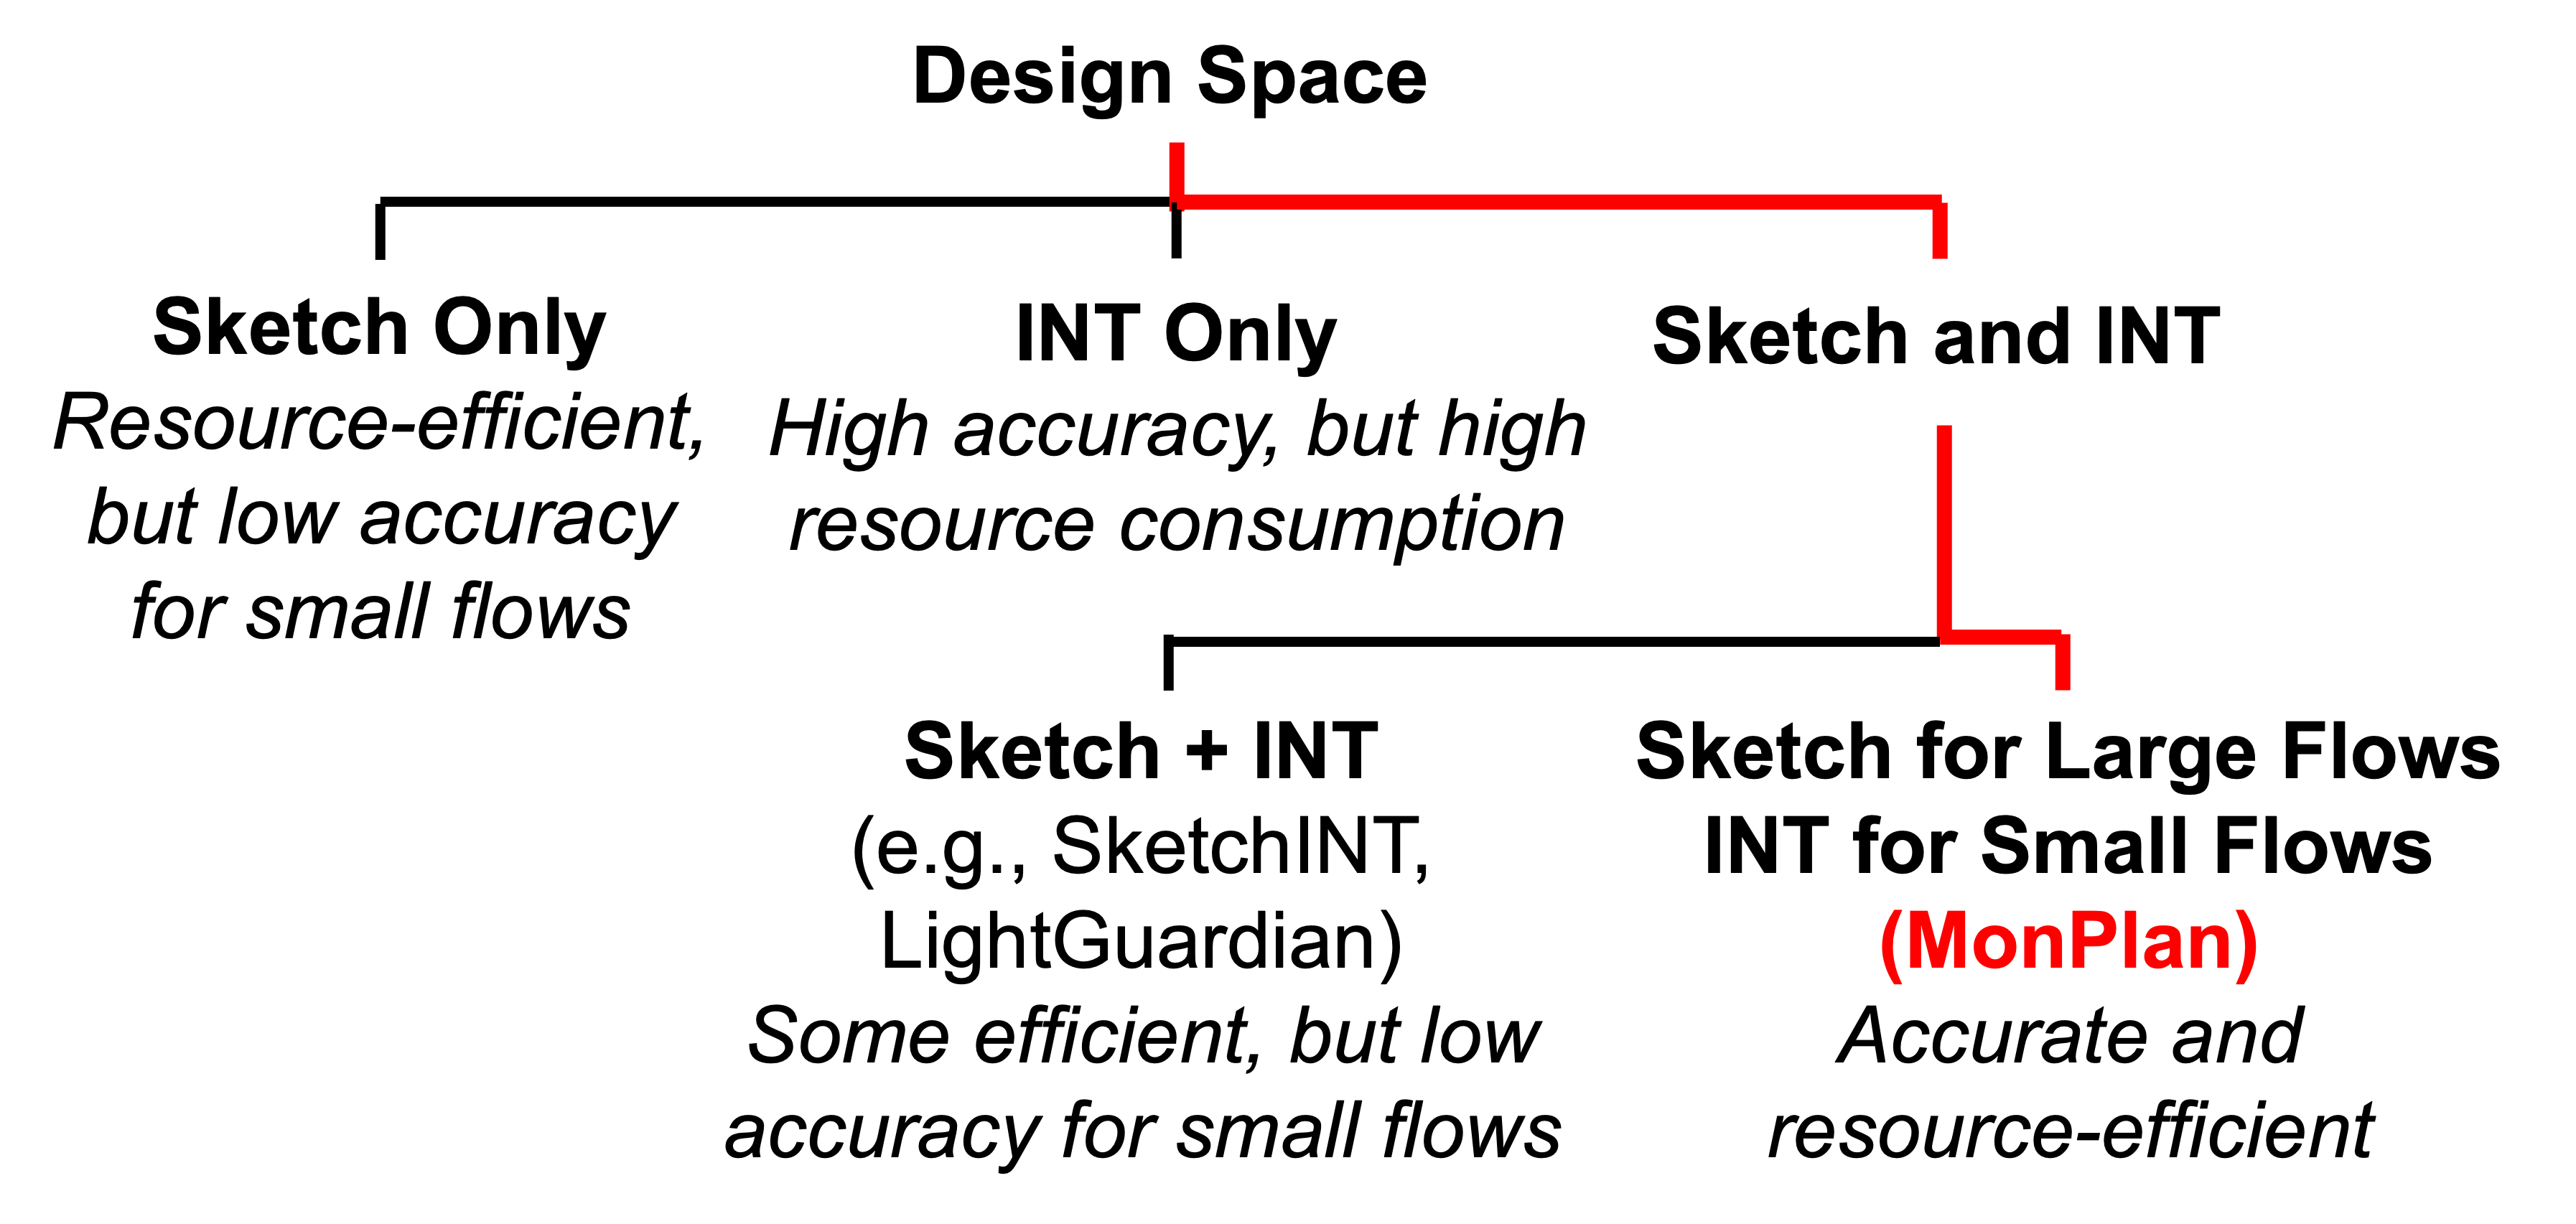
\includegraphics[width=\linewidth]{pics/DesignSpace.png}
    \caption{\sysname explicitly separates the processing of large flows (handled by sketches) and small flows (handled by INT) based on traffic skewness, making it accurate and efficient.}
    \label{DesignSpace}
\end{figure}

\subsection{Our Scope: Network Measurement and Applications}

We first illustrate our scope in this paper. We follow existing studies \cite{namkung2022sketchlib,anup2022hetero,liu2016one} to consider a general architecture of network measurement comprising two planes. In the data plane, switches execute sketches and INT techniques to collect traffic statistics to a cluster of servers that collectively act as the control plane. The control plane runs network management applications that query statistics to identify network events and make decisions. We define relevant terms without loss of generality \cite{liu2024disco,wu2025lemon}:

\begin{itemize}[leftmargin=*]
%
    \item Each packet can be viewed as a tuple of header fields (e.g., IP) and metadata (e.g., packet size and location traversed).
%
    \item Each flow groups the packets that share the same set of header fields and metadata, e.g., the same source IP address. 
%
    \item Traffic statistics, or per-flow statistics, correspond to the flow attributes of interest, e.g., per-flow packet counts. 
%
\end{itemize}

% \noindent With the above terms, we classify network management applications into three classes based on their differences on queries.

% \begin{itemize}[leftmargin=*]
% %
%     \item Volumetric applications, including heavy hitter detection \cite{huang2017sketchvisor}, superspreader detection \cite{tang2019mv}, and DDoS flow detection \cite{liu2021jaqen}, query the size of each flow (e.g., packet or byte counts). 
% %
%     \item Aggregated applications, e.g., traffic cardinality and entropy estimation \cite{liu2016one}, aggregate statistics to summarize all flows. 
% %
%     \item Troubleshooting applications, e.g., path and latency monitoring \cite{ben2020pint,sheng2021deltaint}, query per-flow metadata (e.g., timestamps).
% %
% \end{itemize}

%\noindent Also, since measurements may suffer from errors, the literature introduces several application-level accuracy metrics to evaluate the quality of measurements: the precision, \emph{tp}/(\emph{tp}+\emph{fp}), the recall, \emph{tp}/(\emph{tp}+\emph{fn}), and the F1 score, 2\emph{tp}/(2\emph{tp}+\emph{fp}+\emph{fn}), where \emph{tp}, \emph{fp}, and \emph{fn} denote the number of true positives, false positives, and false negatives, respectively. 

\subsection{Sketches and Limitations}\label{sketches}

Sketches are the approximate algorithms that provide near-optimal accuracy guarantees to the measurement of large flows. Their resource consumption is below a limited budget, making them compatible with resource-constrained switches. Numerous studies \cite{li2016flowradar,yang2018elastic,huang2017sketchvisor,huang2018sketchlearn,liu2016one,huang2021toward,liu2019nitrosketch,zhang2021cocosketch,namkung2022sketchlib} have shown that sketches provide better accuracy-resource tradeoffs for large flows when compared with sampling-based techniques.
% such as NetFlow \cite{netflow}. 
%Note that our work is not to propose new sketches. Instead, we focus on leveraging existing sketches to enable better measurements. 

\para{Limitation 1 (L1):} \emph{Sketches can hardly provide high accuracy for small flows}. Sketches can only use a few memory in their data structures due to switch resource constraints. As a result, the data of large flows and small flows easily collide, resulting in measurement errors. In particular, the measurement of small flows is extremely sensitive to such errors because these flows have very few packets and may be missed entirely or their small counts may be overestimated due to hash collisions. 

% figure a: from nze-sketch background, x = sketches, y = ratio
% figure b: x = the ratio of switches activating INT from 20\% to 100\% (100% = 152 switches), y = number of INT headers, each switch handles 1 Tbps traffic => each packet generates an INT header

We validate our claim with testbed experiments. We consider five sketches and employ them for the application of per-flow packet counting, i.e., the count-min sketch (CM) \cite{cormode2005s}, the count sketch (CS) \cite{charikar2004finding}, the elastic sketch (ES) \cite{yang2018elastic}, SketchLearn (SL) \cite{huang2018sketchlearn}, and UnivMon (UM) \cite{liu2016one}. We consider the de-facto standard traffic traces, CAIDA \cite{caida}, and partition them into two-second intervals, each containing 100\,K flows. Then for each sketch, we allocate 10\,MB to its data structures because this configuration approximates the maximum memory capacity per switch \cite{gupta2018sonata}. 
We measure the ratio of flows with $<10$\% errors in each sketch. Due to space limitations, we report numerical results: all ratios are lower than 50\% because most small flows suffer from non-trivial errors due to memory shortage. 

%If we allocate sufficient memory to each sketch, the accuracy will be improved. However, this is infeasible due to switch constraints. 

Some recent studies have been proposed to tackle the above issue. For example, NZE-sketch \cite{huang2021toward} leverages the theories of compressive sensing to design sketches to approximately record traffic data in switches, and recover original data in the control plane. Moreover, learning-based sketches such as TalentSketch \cite{li2024learning} leverage machine learning models to identify which flows suffer from low measurement accuracy and update sketch data structures in subsequent measurements. However, they exhibit similar issues. First, they need specific sketch design to enforce their optimizations, losing the generality of supporting different types of sketches or network management applications. Second, their recovery or updating strategies require O(10$^2$) seconds, making them unsuitable for a lot of scenarios in which measurements should be made within a few milliseconds. For example, DDoS detection addresses sub-millisecond detection time \cite{liu2021jaqen}. 

\subsection{In-Band Network Telemetry (INT) and Limitations}\label{int}

The core idea of INT is simple yet effective. For each packet, INT orders every switch that the packet traverses to piggyback the information required for measurement onto the packet's INT header. At the egress switch, where packets leave the network, their INT headers are extracted and emitted to the control plane for further analysis. Thus, INT preserves full accuracy for every flow, especially for small flows. 

\para{Limitation 2 (L2):} \emph{INT can bring significant network resource overheads}. Since INT corresponds to per-packet monitoring, it inevitably brings significant overheads to both network bandwidth (for transferring INT headers) and control plane resources (for processing INT headers) given massive packet number. In theory, according to the INT protocol \cite{int}, each switch will add a 12-byte INT header to each packet while the total number of INT headers equals the number of hops traversed by the packet. Given that modern networks transfer Tbps-level traffic, the total number of packets per second is O(10$^9$), corresponding to the number of INT headers to be emitted simultaneously. Hence, although 12\,bytes seem to be small, the accumulation of O(10$^9$) INT headers becomes significant and unacceptable. 

%Figure~1 highlights the impact of number of switches in the network on INT overheads. In detail, we consider the topology of a production network from one of the largest national Internet service providers. This network has 152 switches and 225 links. We vary the ratio of switches activating INT from 20\% to 100\%. We quantify the overheads in terms of number of INT headers to be collected with respect to real-world statistics (e.g., how many packets that a switch processes per second) collected from production. Our results show that even with 20\% switches, INT still introduces non-trivial overheads in terms of bandwidth and computational resources in the control plane. 

To date, many optimizations have been proposed to optimize INT overheads. First, some of them rely on sampling and only invoke INT for sampled packets \cite{tang2019sel,suh2020flexible,kim2018selective,ben2020pint}. Nevertheless, sampling hurts accuracy, especially for small flows with a few packets. Also, the control plane requires a long time for result convergence. Next, INT-path \cite{pan2019int} sends probes to determine the minimum set of non-overlapped paths that INT must measure. But its per-packet monitoring still suffers from high overheads. 
%
Second, some approaches propose to simplify INT information on each packet \cite{ben2020pint,zhao2021lightguardian,sheng2021deltaint}. PINT \cite{ben2020pint} reduces INT metadata via sampling-based global hashing and distributed encoding. But it inherits the issues of sampling. 

\subsection{Limitations of Hybrid Sketch+INT Solutions}\label{hybrid}

Two recent techniques provide hybrid solutions that combine sketches and INT. First, SketchINT \cite{yang2023sketchint} activates INT at data plane switches while leveraging sketches at the control plane to aggregate INT data and simplify subsequent analysis. However, due to its base of INT, it inherits \textbf{L2}. Also, its use of sketches trades the accuracy of small flows for control plane efficiency, leading to \textbf{L1}. Second, LightGuardian \cite{zhao2021lightguardian} uses small sketches to encode INT data in each packet in a compact manner. Hence, it addresses \textbf{L2} because it only requires a few packets to deliver a small amount of sketch data via INT. But given the nature of sketches, it inevitably loses accuracy for small flows, i.e., \textbf{L1}. 

%\para{Takeaways}. Standalone sketches, INT, and strawman sketch-INT hybrid solutions, fail to address \textbf{L1} and \textbf{L2} simultaneously.  


%To maximize resource efficiency, measurement data should be aggressively reduced. But existing techniques \cite{sheng2021deltaint,chen2021mtp,liu2022escala} only consider one type of measurement data and naturally fail to handle the fundamental heterogeneity between sketch data (i.e., sketch counter arrays) and INT data (i.e., INT headers). Also, reducing data must preserve integrity, i.e., 

%For example, many approaches \cite{sheng2021deltaint,chen2021mtp,liu2022escala} only consider one type of measurement data. Thus, they naturally lack a uniform way to reduce heterogeneous data. 

%Traditional static data reduction techniques fail to handle skewed and time-varying traffic patterns, leading to either insufficient compression (wasting bandwidth) or over-aggregation (missing critical details). This is because measurement data scale depends on the flow size: large flows tolerate summarization, while small flows require precision. For example, sketch data alone can be compressed by merging similar values, but INT data may reduce a 1MB sketch update to 100KB during stable periods but fails during traffic shifts (e.g., DDoS onset), where 95\% of counters change simultaneously. Similarly, caching frequent items risks missing ephemeral but critical microburst indicators. This forces inefficient tradeoffs: aggressive reduction distorts small-flow accuracy, while conservative approaches flood control planes during volatility.

%TowerSketch \cite{}

